\documentclass[a4paper,12pt]{letteracdp}

\usepackage[document]{ragged2e}
\usepackage[utf8]{inputenc}
\usepackage[english, italian]{babel}
\usepackage{graphicx}
\usepackage[official]{eurosym}

%Informazioni mittente
\address{
	
\includegraphics[scale=0.40]{logo.png} \\
    \vspace{0.2cm}
    \hspace{0.1cm}
	Gruppo \textit{VRAM Software} \\
}


\signature{
	Vittorio Corrizzato \\
	\textit{Responsabile di Progetto}\\
	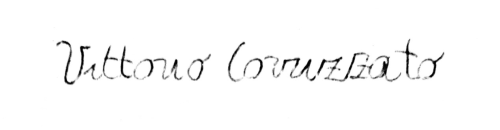
\includegraphics[scale=0.50]{firma-VittorioC.png}
}

\place{Padova}
\date{14 gennaio 2020}

\pagenumbering{gobble}

\begin{document}
\begin{letter}{
		%Informazioni destinatario
		Prof. Vardanega Tullio \\
		Prof. Cardin Riccardo \\
		Dipartimento di Matematica \\
		Università degli Studi di Padova \\
		Via Trieste, 63 \\
		35121 Padova}
	
	\opening{Egregio Prof. Vardanega Tullio, \\ \noindent Egregio Prof. Riccardo Cardin,}
	
	\begin{flushleft}
	Con la presente lettera, il gruppo \textit{VRAM Software} desidera comunicarvi ufficialmente l'impegno alla realizzazione del prodotto \textit{Predire in Grafana}, da voi commissionato e proposto dall'azienda \textit{Zucchetti S.p.A.}
	Le specifiche dell'offerta sono discusse in dettaglio nei documenti allegati:
	\end{flushleft}

	\begin{itemize}
		\item Analisi dei Requisiti v1.1.1
		\item Piano di Qualifica v1.1.1
		\item Piano di Progetto v1.1.1
		\item Norme di Progetto v1.1.1
		\item Studio di Fattibilità v1.1.1
		\item Glossario v1.1.1
		\item Verbale Interno 18-11-2019
		\item Verbale Interno 02-12-2019
		\item Verbale Interno 20-12-2019
		\item Verbale Interno 29-12-2019
		\item Verbale Interno 05-01-2020
		\item Verbale Interno 10-01-2020
		\item Verbale Esterno 18-12-2019
		\item Verbale Esterno 09-01-2020
	\end{itemize}

	\begin{flushleft}
	\noindent Come descritto nel documento Piano di Progetto v.1.1.1, il gruppo si impegna a consegnare il prodotto entro il giorno 11-05-2020, con costo totale preventivato che ammonta a \euro{13341}.
	\\
	
	Rimaniamo a vostra disposizione per eventuali chiarimenti.
	\end{flushleft}

	\closing{Cordiali saluti,}
	
\end{letter}	
\end{document}


